% Options for packages loaded elsewhere
% Options for packages loaded elsewhere
\PassOptionsToPackage{unicode}{hyperref}
\PassOptionsToPackage{hyphens}{url}
\PassOptionsToPackage{dvipsnames,svgnames,x11names}{xcolor}
%
\documentclass[
  letterpaper,
  DIV=11,
  numbers=noendperiod]{scrartcl}
\usepackage{xcolor}
\usepackage{amsmath,amssymb}
\setcounter{secnumdepth}{-\maxdimen} % remove section numbering
\usepackage{iftex}
\ifPDFTeX
  \usepackage[T1]{fontenc}
  \usepackage[utf8]{inputenc}
  \usepackage{textcomp} % provide euro and other symbols
\else % if luatex or xetex
  \usepackage{unicode-math} % this also loads fontspec
  \defaultfontfeatures{Scale=MatchLowercase}
  \defaultfontfeatures[\rmfamily]{Ligatures=TeX,Scale=1}
\fi
\usepackage{lmodern}
\ifPDFTeX\else
  % xetex/luatex font selection
\fi
% Use upquote if available, for straight quotes in verbatim environments
\IfFileExists{upquote.sty}{\usepackage{upquote}}{}
\IfFileExists{microtype.sty}{% use microtype if available
  \usepackage[]{microtype}
  \UseMicrotypeSet[protrusion]{basicmath} % disable protrusion for tt fonts
}{}
\makeatletter
\@ifundefined{KOMAClassName}{% if non-KOMA class
  \IfFileExists{parskip.sty}{%
    \usepackage{parskip}
  }{% else
    \setlength{\parindent}{0pt}
    \setlength{\parskip}{6pt plus 2pt minus 1pt}}
}{% if KOMA class
  \KOMAoptions{parskip=half}}
\makeatother
% Make \paragraph and \subparagraph free-standing
\makeatletter
\ifx\paragraph\undefined\else
  \let\oldparagraph\paragraph
  \renewcommand{\paragraph}{
    \@ifstar
      \xxxParagraphStar
      \xxxParagraphNoStar
  }
  \newcommand{\xxxParagraphStar}[1]{\oldparagraph*{#1}\mbox{}}
  \newcommand{\xxxParagraphNoStar}[1]{\oldparagraph{#1}\mbox{}}
\fi
\ifx\subparagraph\undefined\else
  \let\oldsubparagraph\subparagraph
  \renewcommand{\subparagraph}{
    \@ifstar
      \xxxSubParagraphStar
      \xxxSubParagraphNoStar
  }
  \newcommand{\xxxSubParagraphStar}[1]{\oldsubparagraph*{#1}\mbox{}}
  \newcommand{\xxxSubParagraphNoStar}[1]{\oldsubparagraph{#1}\mbox{}}
\fi
\makeatother

\usepackage{color}
\usepackage{fancyvrb}
\newcommand{\VerbBar}{|}
\newcommand{\VERB}{\Verb[commandchars=\\\{\}]}
\DefineVerbatimEnvironment{Highlighting}{Verbatim}{commandchars=\\\{\}}
% Add ',fontsize=\small' for more characters per line
\usepackage{framed}
\definecolor{shadecolor}{RGB}{241,243,245}
\newenvironment{Shaded}{\begin{snugshade}}{\end{snugshade}}
\newcommand{\AlertTok}[1]{\textcolor[rgb]{0.68,0.00,0.00}{#1}}
\newcommand{\AnnotationTok}[1]{\textcolor[rgb]{0.37,0.37,0.37}{#1}}
\newcommand{\AttributeTok}[1]{\textcolor[rgb]{0.40,0.45,0.13}{#1}}
\newcommand{\BaseNTok}[1]{\textcolor[rgb]{0.68,0.00,0.00}{#1}}
\newcommand{\BuiltInTok}[1]{\textcolor[rgb]{0.00,0.23,0.31}{#1}}
\newcommand{\CharTok}[1]{\textcolor[rgb]{0.13,0.47,0.30}{#1}}
\newcommand{\CommentTok}[1]{\textcolor[rgb]{0.37,0.37,0.37}{#1}}
\newcommand{\CommentVarTok}[1]{\textcolor[rgb]{0.37,0.37,0.37}{\textit{#1}}}
\newcommand{\ConstantTok}[1]{\textcolor[rgb]{0.56,0.35,0.01}{#1}}
\newcommand{\ControlFlowTok}[1]{\textcolor[rgb]{0.00,0.23,0.31}{\textbf{#1}}}
\newcommand{\DataTypeTok}[1]{\textcolor[rgb]{0.68,0.00,0.00}{#1}}
\newcommand{\DecValTok}[1]{\textcolor[rgb]{0.68,0.00,0.00}{#1}}
\newcommand{\DocumentationTok}[1]{\textcolor[rgb]{0.37,0.37,0.37}{\textit{#1}}}
\newcommand{\ErrorTok}[1]{\textcolor[rgb]{0.68,0.00,0.00}{#1}}
\newcommand{\ExtensionTok}[1]{\textcolor[rgb]{0.00,0.23,0.31}{#1}}
\newcommand{\FloatTok}[1]{\textcolor[rgb]{0.68,0.00,0.00}{#1}}
\newcommand{\FunctionTok}[1]{\textcolor[rgb]{0.28,0.35,0.67}{#1}}
\newcommand{\ImportTok}[1]{\textcolor[rgb]{0.00,0.46,0.62}{#1}}
\newcommand{\InformationTok}[1]{\textcolor[rgb]{0.37,0.37,0.37}{#1}}
\newcommand{\KeywordTok}[1]{\textcolor[rgb]{0.00,0.23,0.31}{\textbf{#1}}}
\newcommand{\NormalTok}[1]{\textcolor[rgb]{0.00,0.23,0.31}{#1}}
\newcommand{\OperatorTok}[1]{\textcolor[rgb]{0.37,0.37,0.37}{#1}}
\newcommand{\OtherTok}[1]{\textcolor[rgb]{0.00,0.23,0.31}{#1}}
\newcommand{\PreprocessorTok}[1]{\textcolor[rgb]{0.68,0.00,0.00}{#1}}
\newcommand{\RegionMarkerTok}[1]{\textcolor[rgb]{0.00,0.23,0.31}{#1}}
\newcommand{\SpecialCharTok}[1]{\textcolor[rgb]{0.37,0.37,0.37}{#1}}
\newcommand{\SpecialStringTok}[1]{\textcolor[rgb]{0.13,0.47,0.30}{#1}}
\newcommand{\StringTok}[1]{\textcolor[rgb]{0.13,0.47,0.30}{#1}}
\newcommand{\VariableTok}[1]{\textcolor[rgb]{0.07,0.07,0.07}{#1}}
\newcommand{\VerbatimStringTok}[1]{\textcolor[rgb]{0.13,0.47,0.30}{#1}}
\newcommand{\WarningTok}[1]{\textcolor[rgb]{0.37,0.37,0.37}{\textit{#1}}}

\usepackage{longtable,booktabs,array}
\newcounter{none} % for unnumbered tables
\usepackage{calc} % for calculating minipage widths
% Correct order of tables after \paragraph or \subparagraph
\usepackage{etoolbox}
\makeatletter
\patchcmd\longtable{\par}{\if@noskipsec\mbox{}\fi\par}{}{}
\makeatother
% Allow footnotes in longtable head/foot
\IfFileExists{footnotehyper.sty}{\usepackage{footnotehyper}}{\usepackage{footnote}}
\makesavenoteenv{longtable}
\usepackage{graphicx}
\makeatletter
\newsavebox\pandoc@box
\newcommand*\pandocbounded[1]{% scales image to fit in text height/width
  \sbox\pandoc@box{#1}%
  \Gscale@div\@tempa{\textheight}{\dimexpr\ht\pandoc@box+\dp\pandoc@box\relax}%
  \Gscale@div\@tempb{\linewidth}{\wd\pandoc@box}%
  \ifdim\@tempb\p@<\@tempa\p@\let\@tempa\@tempb\fi% select the smaller of both
  \ifdim\@tempa\p@<\p@\scalebox{\@tempa}{\usebox\pandoc@box}%
  \else\usebox{\pandoc@box}%
  \fi%
}
% Set default figure placement to htbp
\def\fps@figure{htbp}
\makeatother





\setlength{\emergencystretch}{3em} % prevent overfull lines

\providecommand{\tightlist}{%
  \setlength{\itemsep}{0pt}\setlength{\parskip}{0pt}}



 
\usepackage[]{biblatex}


\KOMAoption{captions}{tableheading}
\makeatletter
\@ifpackageloaded{tcolorbox}{}{\usepackage[skins,breakable]{tcolorbox}}
\@ifpackageloaded{fontawesome5}{}{\usepackage{fontawesome5}}
\definecolor{quarto-callout-color}{HTML}{909090}
\definecolor{quarto-callout-note-color}{HTML}{0758E5}
\definecolor{quarto-callout-important-color}{HTML}{CC1914}
\definecolor{quarto-callout-warning-color}{HTML}{EB9113}
\definecolor{quarto-callout-tip-color}{HTML}{00A047}
\definecolor{quarto-callout-caution-color}{HTML}{FC5300}
\definecolor{quarto-callout-color-frame}{HTML}{acacac}
\definecolor{quarto-callout-note-color-frame}{HTML}{4582ec}
\definecolor{quarto-callout-important-color-frame}{HTML}{d9534f}
\definecolor{quarto-callout-warning-color-frame}{HTML}{f0ad4e}
\definecolor{quarto-callout-tip-color-frame}{HTML}{02b875}
\definecolor{quarto-callout-caution-color-frame}{HTML}{fd7e14}
\makeatother
\makeatletter
\@ifpackageloaded{caption}{}{\usepackage{caption}}
\AtBeginDocument{%
\ifdefined\contentsname
  \renewcommand*\contentsname{Table of contents}
\else
  \newcommand\contentsname{Table of contents}
\fi
\ifdefined\listfigurename
  \renewcommand*\listfigurename{List of Figures}
\else
  \newcommand\listfigurename{List of Figures}
\fi
\ifdefined\listtablename
  \renewcommand*\listtablename{List of Tables}
\else
  \newcommand\listtablename{List of Tables}
\fi
\ifdefined\figurename
  \renewcommand*\figurename{Figure}
\else
  \newcommand\figurename{Figure}
\fi
\ifdefined\tablename
  \renewcommand*\tablename{Table}
\else
  \newcommand\tablename{Table}
\fi
}
\@ifpackageloaded{float}{}{\usepackage{float}}
\floatstyle{ruled}
\@ifundefined{c@chapter}{\newfloat{codelisting}{h}{lop}}{\newfloat{codelisting}{h}{lop}[chapter]}
\floatname{codelisting}{Listing}
\newcommand*\listoflistings{\listof{codelisting}{List of Listings}}
\makeatother
\makeatletter
\makeatother
\makeatletter
\@ifpackageloaded{caption}{}{\usepackage{caption}}
\@ifpackageloaded{subcaption}{}{\usepackage{subcaption}}
\makeatother
\usepackage{bookmark}
\IfFileExists{xurl.sty}{\usepackage{xurl}}{} % add URL line breaks if available
\urlstyle{same}
% fallback for those not using the hyperref driver hyperxmp:
\makeatletter
\@ifundefined{xmpquote}{\newcommand{\xmpquote}[1]{#1}}{}
\makeatother
\hypersetup{
  pdftitle={Leetcode: Data Structure and Algorithms},
  pdfauthor={Rafiq Islam},
  colorlinks=true,
  linkcolor={blue},
  filecolor={Maroon},
  citecolor={Blue},
  urlcolor={Blue},
  pdfcreator={LaTeX via pandoc}}


\title{Leetcode: Data Structure and Algorithms}
\author{Rafiq Islam}
\date{}
\begin{document}
\maketitle

\renewcommand*\contentsname{Table of contents}
{
\setcounter{tocdepth}{4}
\tableofcontents
}

\subsection{Binary Search}\label{binary-search}

\begin{tcolorbox}[enhanced jigsaw, arc=.35mm, bottomrule=.15mm, breakable, colback=white, colframe=quarto-callout-note-color-frame, left=2mm, leftrule=.75mm, opacityback=0, rightrule=.15mm, toprule=.15mm]

\vspace{-3mm}\textbf{Problem 1: Leetcode 69: Sqrt(x)}\vspace{3mm}

Given a non-negative integer, \(x\), return the square root of \(x\)
rounded down to the nearest integer. The returned integer should be
non-negative as well.

You may not use any built-in exponent function. For example,
\texttt{x**0.5} in python.

Example:

\begin{Shaded}
\begin{Highlighting}[]
\NormalTok{Input: x}\OperatorTok{=}\DecValTok{4}
\NormalTok{Output: }\DecValTok{2}  

\NormalTok{Input: x}\OperatorTok{=}\DecValTok{8}
\NormalTok{Output: }\DecValTok{2}
\end{Highlighting}
\end{Shaded}

Explanation: Square root of 4 is 2 and square root of 8 is 2.8284. But
we need to round down to any fraction. Therefore, the square root of 8
is also 2.

\textbf{Solution:}

The square root of any number \(x\ge 0\) is less than or equal to \(x\).
The brute force solution to this would be \(\mathcal{O}(\sqrt{n})\).
Because, say \(x=8\), then

for \(i=1\) to 8: \begin{align*}
  1^2 & = 1 <8 \\
  2^2 & = 4 <8\\
  3^2 & = 9 >8
\end{align*}

\pandocbounded{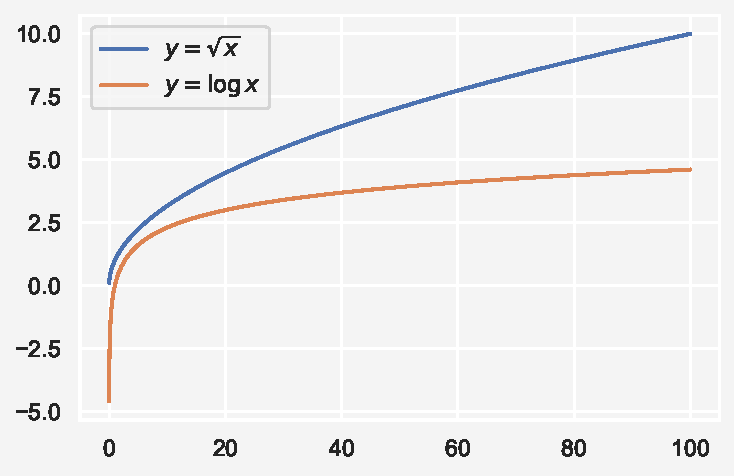
\includegraphics[keepaspectratio]{index_files/figure-pdf/cell-2-output-1.pdf}}

In contrast, if we explore binary search then the time complexity
reduces to \(\mathcal{O}(\log{n})\). Say the square root is \(s\) which
is the middle value in the range of 1 to \(x\). Then if \(s^2>x\), we
search for the root in the left half. Otherwise, if \(s^2<x\) then we
search the right side. However, when \(s^2<x\), then \(s\) is a possible
candidate for the square root.

\emph{Algorithm:}

\begin{enumerate}
\def\labelenumi{\arabic{enumi}.}
\tightlist
\item
  set left value \(l= 0\), right value \(r= x\)\\
\item
  Compute the middle value \(m=l+(r-l)/2\)\\
\item
  If \(m^2 > x\) then search the left side: set \(r=m-1\)\\
\item
  If \(m^2 < x\) then search the right side: set \(l=m+1\)
\end{enumerate}

\begin{Shaded}
\begin{Highlighting}[]
\KeywordTok{def}\NormalTok{ square\_root(x):}
\NormalTok{  l, r }\OperatorTok{=} \DecValTok{0}\NormalTok{, x }
\NormalTok{  sq }\OperatorTok{=} \DecValTok{0}
  \ControlFlowTok{while}\NormalTok{ l}\OperatorTok{\textless{}=}\NormalTok{r:}
\NormalTok{    m }\OperatorTok{=}\NormalTok{ l }\OperatorTok{+}\NormalTok{ (r}\OperatorTok{{-}}\NormalTok{l)}\OperatorTok{//}\DecValTok{2} 
    \ControlFlowTok{if}\NormalTok{ m}\OperatorTok{**}\DecValTok{2} \OperatorTok{\textgreater{}}\NormalTok{ x:}
\NormalTok{      r}\OperatorTok{=}\NormalTok{ m}\OperatorTok{{-}}\DecValTok{1}
    \ControlFlowTok{elif}\NormalTok{ m}\OperatorTok{**}\DecValTok{2} \OperatorTok{\textless{}}\NormalTok{ x:}
\NormalTok{      l }\OperatorTok{=}\NormalTok{ m}\OperatorTok{+}\DecValTok{1} 
\NormalTok{      sq }\OperatorTok{=}\NormalTok{ m}
    \ControlFlowTok{else}\NormalTok{:}
      \ControlFlowTok{return}\NormalTok{ m  }
  \ControlFlowTok{return}\NormalTok{ sq }
      
\BuiltInTok{print}\NormalTok{(square\_root(}\DecValTok{6}\NormalTok{))}
\end{Highlighting}
\end{Shaded}

\begin{verbatim}
2
\end{verbatim}

\end{tcolorbox}

\subsection{Array}\label{array}

\begin{tcolorbox}[enhanced jigsaw, arc=.35mm, bottomrule=.15mm, breakable, colback=white, colframe=quarto-callout-note-color-frame, left=2mm, leftrule=.75mm, opacityback=0, rightrule=.15mm, toprule=.15mm]

\vspace{-3mm}\textbf{Problem 1: Intersection of two sets}\vspace{3mm}

Say, we are given two sets \(A=[2,3,5,6,8]\) and \(B=[4,6,8]\). We want
to find the intersection of the elements in these sets.

\begin{Shaded}
\begin{Highlighting}[]
\KeywordTok{def}\NormalTok{ intersection\_of\_two\_sets(A,B):}
\NormalTok{  set\_a }\OperatorTok{=} \BuiltInTok{set}\NormalTok{(A)}
  \ControlFlowTok{return}\NormalTok{ [b }\ControlFlowTok{for}\NormalTok{ b }\KeywordTok{in}\NormalTok{ B }\ControlFlowTok{if}\NormalTok{ b }\KeywordTok{in}\NormalTok{ set\_a]}

\NormalTok{A }\OperatorTok{=}\NormalTok{ [}\DecValTok{2}\NormalTok{,}\DecValTok{3}\NormalTok{,}\DecValTok{5}\NormalTok{,}\DecValTok{6}\NormalTok{,}\DecValTok{8}\NormalTok{]}
\NormalTok{B }\OperatorTok{=}\NormalTok{ [}\DecValTok{4}\NormalTok{,}\DecValTok{6}\NormalTok{,}\DecValTok{8}\NormalTok{]}
\BuiltInTok{print}\NormalTok{(intersection\_of\_two\_sets(A,B))}
\end{Highlighting}
\end{Shaded}

{[}6, 8{]}

\end{tcolorbox}

\begin{tcolorbox}[enhanced jigsaw, arc=.35mm, bottomrule=.15mm, breakable, colback=white, colframe=quarto-callout-note-color-frame, left=2mm, leftrule=.75mm, opacityback=0, rightrule=.15mm, toprule=.15mm]

\vspace{-3mm}\textbf{Problem 2: Histogram from a given array and bin number}\vspace{3mm}

Say, we are given an array \(A=[1,2,2,3,3,3,4,4,4,4,5,5,5,5,5]\) and
number of bins. We want to

\begin{Shaded}
\begin{Highlighting}[]
\KeywordTok{def}\NormalTok{ generate\_histogram(A, num\_bins):}
\NormalTok{  min\_value }\OperatorTok{=} \BuiltInTok{min}\NormalTok{(A)}
\NormalTok{  max\_value }\OperatorTok{=} \BuiltInTok{max}\NormalTok{(A)}
\NormalTok{  bin\_width }\OperatorTok{=}\NormalTok{ (max\_value}\OperatorTok{{-}}\NormalTok{min\_value)}\OperatorTok{/}\NormalTok{num\_bins}
\end{Highlighting}
\end{Shaded}

\end{tcolorbox}

\begin{tcolorbox}[enhanced jigsaw, arc=.35mm, bottomrule=.15mm, breakable, colback=white, colframe=quarto-callout-note-color-frame, left=2mm, leftrule=.75mm, opacityback=0, rightrule=.15mm, toprule=.15mm]

\vspace{-3mm}\textbf{Problem 3: LeetCode 1: Two Sum}\vspace{3mm}

Say we have an array of integers \(A=[2,1,5,3]\) and a target
\texttt{target=4}. We want to find the sum of two elements in the array
that equals the target. We want to return the indices of the two
elements. The best possible way to solve this problem is to use a
hashmap. We can store the elements of the array in a hashmap and check
if the complement of the current element exists in the hashmap. If it
does, we return the indices of the two elements.

\textbf{Time Complexity:} \(\mathcal{O}(n)\) where \(n\) is the length
of the array.\\
\textbf{Space Complexity:} \(\mathcal{O}(n)\) where \(n\) is the length
of the array.

\begin{Shaded}
\begin{Highlighting}[]
\KeywordTok{def}\NormalTok{ two\_sum(nums, target):}
\NormalTok{  prevMap }\OperatorTok{=}\NormalTok{ \{\} }\CommentTok{\# Value : Index}
  \ControlFlowTok{for}\NormalTok{ i, n }\KeywordTok{in} \BuiltInTok{enumerate}\NormalTok{(nums):}
\NormalTok{    diff }\OperatorTok{=}\NormalTok{ target }\OperatorTok{{-}}\NormalTok{ n}
    \ControlFlowTok{if}\NormalTok{ diff }\KeywordTok{in}\NormalTok{ prevMap:}
      \ControlFlowTok{return}\NormalTok{ [prevMap[diff], i]}
\NormalTok{    prevMap[n] }\OperatorTok{=}\NormalTok{ i}
  \ControlFlowTok{return}\NormalTok{ []}

\NormalTok{nums }\OperatorTok{=}\NormalTok{ [}\DecValTok{2}\NormalTok{,}\DecValTok{1}\NormalTok{,}\DecValTok{5}\NormalTok{,}\DecValTok{3}\NormalTok{]}
\NormalTok{target }\OperatorTok{=} \DecValTok{4}
\BuiltInTok{print}\NormalTok{(two\_sum(nums, target))}
\end{Highlighting}
\end{Shaded}

{[}1, 3{]}

\end{tcolorbox}

\subsection{String}\label{string}

\begin{tcolorbox}[enhanced jigsaw, arc=.35mm, bottomrule=.15mm, breakable, colback=white, colframe=quarto-callout-note-color-frame, left=2mm, leftrule=.75mm, opacityback=0, rightrule=.15mm, toprule=.15mm]

\vspace{-3mm}\textbf{Problem 1: Leetcode 242: Valid Anagram}\vspace{3mm}

Given two strings \texttt{s} and \texttt{t}, return \texttt{true} if
\texttt{t} is an \emph{anagram} of \texttt{s}, and \texttt{false}
\emph{otherwise}

Example: Input: \texttt{s="anagram"}, \texttt{t="nagaram"} Output:
\texttt{true}

Since the word \texttt{anagram} has 3 a's, 1 n, 1 g, 1 r, and 1 m and
\texttt{nagaram} has exactly the same number of the same alphabets,
therefore they are anagram of each other.

Example: Input: \texttt{s="rat"}, \texttt{t="cat"} Output:
\texttt{false}

Since the word \texttt{rat} has 1 r, 1 a, and 1 t but \texttt{cat} has 2
elements same as \texttt{rat} but one element different. Therefore the
answer is false.

Note that, they both have the same length.

\textbf{Constraints:}

\begin{itemize}
\tightlist
\item
  \(1\le s\).length, \(t\).length \(\le 5\times 10^4\)\\
\item
  \texttt{s} and \texttt{t} consists of lowercase English letters
\end{itemize}

\textbf{Solution:}\\
We can use \texttt{hasmap} to solve this problem. Basically, we will
create two hasmaps for two words and match the keys and values of the
hasmaps. If they are equal then it's an anagram, otherwise not.

\begin{Shaded}
\begin{Highlighting}[]
\KeywordTok{def}\NormalTok{ isAnagram(s,t):}
  \ControlFlowTok{if} \BuiltInTok{len}\NormalTok{(s) }\OperatorTok{!=} \BuiltInTok{len}\NormalTok{(t):}
    \ControlFlowTok{return} \VariableTok{False} 
  
\NormalTok{  hash\_s, hash\_t }\OperatorTok{=}\NormalTok{ \{\}, \{\}}
  \ControlFlowTok{for}\NormalTok{ i }\KeywordTok{in} \BuiltInTok{range}\NormalTok{(}\BuiltInTok{len}\NormalTok{(s)):}
\NormalTok{    hash\_s[s[i]] }\OperatorTok{=} \DecValTok{1} \OperatorTok{+}\NormalTok{ hash\_s.get(s[i],}\DecValTok{0}\NormalTok{)  }\CommentTok{\# get function collects the key and values.}
\NormalTok{    hash\_t[t[i]] }\OperatorTok{=} \DecValTok{1} \OperatorTok{+}\NormalTok{ hash\_t.get(t[i],}\DecValTok{0}\NormalTok{)  }\CommentTok{\# if there\textquotesingle{}s no key, 0 is the default value}
  
  \ControlFlowTok{for}\NormalTok{ c }\KeywordTok{in}\NormalTok{ hash\_s:}
    \ControlFlowTok{if}\NormalTok{ hash\_s[c] }\OperatorTok{!=}\NormalTok{ hash\_t.get(c,}\DecValTok{0}\NormalTok{):       }\CommentTok{\# Here, get function ensures there is no }
      \ControlFlowTok{return} \VariableTok{False}                         \CommentTok{\# key error}
  \ControlFlowTok{return} \VariableTok{True}

\NormalTok{s }\OperatorTok{=} \StringTok{"anagram"}
\NormalTok{t }\OperatorTok{=} \StringTok{"nagaram"}

\BuiltInTok{print}\NormalTok{(isAnagram(s,t))}

\NormalTok{u }\OperatorTok{=} \StringTok{"rat"}

\BuiltInTok{print}\NormalTok{(isAnagram(s,u))}
\end{Highlighting}
\end{Shaded}

\begin{verbatim}
True
False
\end{verbatim}

In the above code:

\begin{Shaded}
\begin{Highlighting}[]
\NormalTok{hash\_s, hash\_t }\OperatorTok{=}\NormalTok{ \{\}, \{\}}
  \ControlFlowTok{for}\NormalTok{ i }\KeywordTok{in} \BuiltInTok{range}\NormalTok{(}\BuiltInTok{len}\NormalTok{(s)):}
\NormalTok{    hash\_s[s[i]] }\OperatorTok{=} \DecValTok{1} \OperatorTok{+}\NormalTok{ hash\_s.get(s[i],}\DecValTok{0}\NormalTok{)  }
\NormalTok{    hash\_t[t[i]] }\OperatorTok{=} \DecValTok{1} \OperatorTok{+}\NormalTok{ hash\_t.get(t[i],}\DecValTok{0}\NormalTok{)  }
\end{Highlighting}
\end{Shaded}

It makes the following hasmaps:

{\def\LTcaptype{none} % do not increment counter
\begin{longtable}[]{@{}cccc@{}}
\toprule\noalign{}
& s & & t \\
\midrule\noalign{}
\endhead
\bottomrule\noalign{}
\endlastfoot
Key & Value & Key & Value \\
a & 3 & a & 3 \\
n & 1 & n & 1 \\
g & 1 & g & 1 \\
r & 1 & r & 1 \\
m & 1 & m & 1 \\
\end{longtable}
}

\textbf{Time and Space Complexity:}\\
Time complexity \(\mathcal{O}(m+n)\) where \(m\) and \(n\) are the
length of \texttt{s} and \texttt{t} and memory complexity is the same
\(\mathcal{O}(m+n)\)

Optimization: Can we solve the problem in \(\mathcal{O}(1)\)? If we
assume sort doesn't require extra space, then

\begin{Shaded}
\begin{Highlighting}[]
\KeywordTok{def}\NormalTok{ isAnagram(s,t):}
  \ControlFlowTok{return} \BuiltInTok{sorted}\NormalTok{(s)}\OperatorTok{==} \BuiltInTok{sorted}\NormalTok{(t)}

\NormalTok{s}\OperatorTok{=} \StringTok{"anagram"}
\NormalTok{t}\OperatorTok{=} \StringTok{"nagaram"}

\BuiltInTok{print}\NormalTok{(isAnagram(s,t))}
\end{Highlighting}
\end{Shaded}

\begin{verbatim}
True
\end{verbatim}

\end{tcolorbox}

\subsection{Reference}\label{reference}

All my solutions here are based on the solutions found from
\href{https://www.youtube.com/c/neetcode}{NeetCode}.


\printbibliography



\end{document}
